\documentclass[12pt]{article}

\usepackage[margin=1in]{geometry}
\usepackage{times}

\usepackage{graphicx}
\usepackage{fancyhdr}
\usepackage{enumitem}
\usepackage{setspace}
\usepackage{xcolor}

% Define a new color for the footer background
\definecolor{footerblue}{RGB}{46,116,181}

\renewcommand{\headrulewidth}{0pt}
\fancypagestyle{headerstyle}{
	\fancyhf{}
	\fancyhead[L]{\textit{\textbf{System Requirement Specification for Malayalam Parser for Dataset Creation}}}
	\fancyhead[R]{\textit{\textbf{Page \thepage}}}
	\fancyfoot[L]{\colorbox{footerblue}{\textcolor{white}{\textit{\textbf{\quad Department of Computer Science and Engineering, RSET\hspace{0.36\linewidth}}}}}}
	\fancyfoot[R]{\colorbox{footerblue}{\textcolor{white}{\textit{\textbf{\thepage}}}}}
}

\pagestyle{empty}
\setstretch{1.5}

\hyphenpenalty=10000
\hbadness=10000



\begin{document}
	
	%\raggedright
	
	\begin{figure}[t]
		\centering
		
\includegraphics[width=4cm]{RSET.png}
		\bigskip
	\end{figure}
	
	
	\begin{center}
		
		\setstretch{1.5}
		
		\textbf{\textit{
				{\fontsize{16pt}{19.2pt}\selectfont
					Software Requirement Specification}}\medskip
			{\fontsize{14pt}{16.8pt}\selectfont
				\\On\medskip\\Malayalam Parser For Dataset Creation}
		}
		
		
		\vspace{1cm}
		
		\setstretch{2.0}
		
		{\fontsize{14pt}{16.8pt}\selectfont
			\textbf{
				By\\
				Fathima Jennath (U2103089)\\
				Gautham C Sudheer(U2103092)\\
				Godwin Gino (U2103096)\\
				Mohammed Basil (U2103139)
			}
			
			\vspace{2cm}
			
			\setstretch{1.5}
			
			\textbf{
				Under the guidance of\\
				Dr. Mary Priya Sebastian\\
			}
			
			\bigskip
			
			\setstretch{1.2}
			
			\textbf{
				Department of Computer Science and Engineering\\
				Rajagiri School of Engineering \& Technology (Autonomous)\\
				(Parent University: APJ Abdul Kalam Technological University)\\
				Rajagiri Valley, Kakkanad, Kochi, 682039\\
				March 2024
			}
		}   
		
	\end{center}
	
	\newpage
	
	\begin{center}
		
		\setstretch{2.0}
		
		\textbf{\textit{
				{\fontsize{16pt}{19.2pt}\selectfont
					Software Requirement Specification}}\medskip
			{\fontsize{14pt}{16.8pt}\selectfont
				\\On\medskip\\Malayalam Parser For Dataset Creation}
		}
		
		\bigskip
		
		{\setstretch{4.0}
			
			\textbf{{\fontsize{14pt}{16.8pt}\selectfont Prepared By\\}}
			
			U2103089 Fathima Jennath\\
			U2103092 Gautham C Sudheer\\
			U2103096 Godwin Gino\\
			U2103139 Mohammed Basil\\
		}
	
		\bigskip \bigskip \bigskip
	
		\setstretch{1.5}
	
		{\fontsize{16pt}{19.2pt}\selectfont \textbf{Guided By: } Dr. Mary Priya Sebastain\\
		\hspace{1.8cm}Associate Professor\\
		\hspace{5.2cm}Dept. of Computer Science, RSET\\}
		
	\end{center}
	
	\newpage
	\pagestyle{headerstyle}
	
	\tableofcontents
	
	\newpage
	\setcounter{page}{1}
	
	\section{Introduction}
	
	\subsection{Purpose}
	This Software Requirements Specification (SRS) document outlines the specifications for
	developing a Malayalam Parser. The goal is to create an NLP-based system capable of
	accurately parsing and understanding Malayalam text data. This document covers
	functional and non-functional requirements, system scope, and serves as a communication
	tool between stakeholders.
	
	\begin{itemize}[label=-]
		\item The Malayalam Parser system will focus primarily on analyzing and parsing written text in the Malayalam language.
		\item Initially, the system will target general-purpose parsing tasks but can be extended to handle domain-specific or specialized parsing tasks in the future.
		\item The scope includes the development of necessary algorithms, data structures and linguistic resources required for accurate parsing of Malayalam text.
	\end{itemize}
	
	\subsection{Product Scope}
	The Malayalam Parser is a smart tool that understands written Malayalam text. It breaks
	down sentences to figure out their grammar, structure, and meaning using advanced
	language processing techniques. It helps with tasks like identifying different parts of
	speech, understanding how sentences are put together, and analyzing the overall meaning
	of text.\\
	The Malayalam Parser directly contributes to corporate goals and business strategies by
	enabling:
	
	\begin{itemize}[label=-]
		\item \textbf{Effective Communication:} By accurately parsing Malayalam text, the tool facilitates clear communication with Malayalam-speaking audiences, supporting
		market expansion and customer engagement.
		
		\item \textbf{Informed Decision-Making:} Extracting insights from Malayalam text aids in	data-driven decision-making, enhancing strategic planning and execution.
		
		\item \textbf{Innovation:} Investment in language processing technologies demonstrates innovation, ensuring the organization remains competitive and adaptable to technological advancements. The Vision and Scope document typically provides an	overarching vision for the project, outlines its objectives, scope, and key	stakeholders, and describes how the project aligns with organizational goals and strategies. By referring to this document, stakeholders can gain a comprehensive understanding of the project's vision, objectives, and scope without unnecessary	repetition of information.
	\end{itemize}

	\section{Overall Description}
	
	\subsection{Product Perspective}
	This software represents a new, standalone product
	developed to fulfill the crucial task of parsing and analyzing Malayalam language text.
	Unlike existing systems or components, this software is designed from the ground up to
	specialize in the intricacies of Malayalam language parsing, catering to the specific needs
	of users requiring accurate linguistic analysis in Malayalam.\\
	The Malayalam Parser software does not belong to a product family but serves as an
	independent solution, tailored specifically for parsing Malayalam text. It is not intended as
	a replacement for existing systems but rather as a complementary tool to enhance
	language processing capabilities in Malayalam. While it operates autonomously, it may
	interface with other systems or applications, such as text input sources or linguistic
	databases, to facilitate seamless integration within broader linguistic analysis frameworks.
	This section does not include a diagram but provides a detailed understanding of the
	software's context within the larger system landscape. It emphasizes the software's role as a standalone entity dedicated to Malayalam language parsing, with potential interfaces to
	external systems for enhanced functionality and interoperability.
	
	\begin{figure}[t]
		\centering
		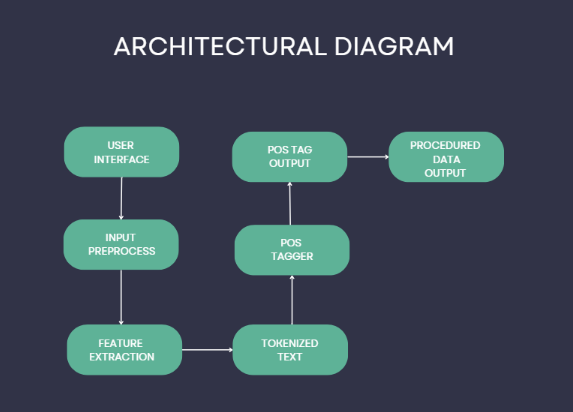
\includegraphics[width=10cm]{architecture.png}
		\bigskip
	\end{figure}
	
	\newpage
	\subsection{Product Functions}
	\textbf{Major Functions of the Malayalam Parser:}
	
	\begin{itemize}[label=-]
		\item Parse and analyze Malayalam language text to identify linguistic components such as
		words, phrases, and sentences.
		\item Determine grammatical structure, syntax, and semantics of Malayalam sentences to
		facilitate accurate linguistic analysis.
		\item Provide functionality for part-of-speech tagging, syntactic parsing, and semantic
		analysis tailored for the Malayalam language.
		\item Support for handling compound words, inflections, and variations in word forms
		commonly found in Malayalam text.
		\item Resolve ambiguity in sentence structure and meaning to ensure precise linguistic
		analysis.
		\item Interface with external systems or applications, such as text input sources or linguistic
		databases, for data integration and enhanced functionality within broader linguistic
		analysis frameworks.
	\end{itemize}

	\subsection{Operating Environment}
	For creating the Malayalam Parser, the operating environment encompasses the following
	specifications:\\
	\textbf{Hardware Platform}
	
	\begin{itemize}[label=-]
		\item The software should be compatible with standard computing hardware commonly
		used for software development and deployment.
		\item Minimum hardware requirements include a modern processor (e.g., Intel Core i5 or
		equivalent), sufficient RAM (at least 4GB), and available storage space for software
		installation and data processing.
	\end{itemize}

	\textbf{Operating System and Versions}
	
	\begin{itemize}[label=-]
		\item The software should be compatible with popular operating systems used for
		software development and deployment, including Windows, macOS, and Linux
		distributions.
		\item Specific operating system versions supported include:
		\item Windows 10 or later
		\item MacOS 10.13 High Sierra or later
		\item Ubuntu 18.04 LTS or later
	\end{itemize}
	
	\textbf{Software Components and Applications}
	
	\begin{itemize}[label=-]
		\item The Malayalam Parser may require integration with various software components and applications for development, testing, and deployment purposes.
		\item Development tools such as Python (version 3.6 or later), Java Development Kit (JDK), or other programming languages and frameworks suitable for NLP development may be necessary.
		\item Libraries and frameworks for natural language processing, such as NLTK (Natural Language Toolkit), spacey or TensorFlow, may be utilized.
		\item Database systems such as SQLite, PostgreSQL, or MongoDB may be employed for data storage and retrieval if necessary.
	\end{itemize}
	
	\subsection{Design and Implementation Constraints}
	The development of the Malayalam Parser is subject to various constraints and limitations, including:
	
	\begin{itemize}[label=-]
		\item \textbf{Corporate or Regulatory Policies:} Compliance with data protection regulations
		and privacy policies is mandatory. The Malayalam Parser must adhere to all
		applicable laws and regulations governing the handling of user data and privacy.
		\item \textbf{Hardware Limitations:} The software must be optimized to operate within
		hardware limitations, including timing and memory constraints. Performance
		optimizations are crucial to ensure efficient operation across different hardware
		configuration.
		\item \textbf{Interfaces to Other Applications:} Compatibility with external applications or
		systems is essential for seamless integration. The Malayalam Parser must support
		standard interfaces and data formats to facilitate interoperability with other
		language processing tools or databases.
		\item \textbf{Specific Technologies, Tools, and Databases:} The use of specific technologies,
		tools, and databases may be mandated by project requirements or organizational
		standards. Developers must adhere to designated technologies and tools approved
		for the project.
		\item \textbf{Language Requirements:} The Malayalam Parser must be designed and
		implemented to meet the linguistic complexities of the Malayalam language. This
		includes handling unique grammar rules, character encoding, and text processing
		requirements inherent to Malayalam.
		\item \textbf{Security Considerations:} Security measures such as encryption, access control,
		and data integrity must be incorporated into the design and implementation of the
		Malayalam Parser to safeguard against security threats and vulnerabilities.
		\item \textbf{Design Conventions and Programming Standards:} Adherence to design
		conventions, programming standards, and coding guidelines is paramount.
		Developers must follow established best practices and organizational standards to
		ensure maintainability, readability, and consistency of the codebase.
	\end{itemize}

	\subsection{Assumptions and Dependencies}
	\begin{enumerate}
		\item \textbf{Third-Party or Commercial Components:} It is assumed that the development of
		the Malayalam Parser will not heavily rely on third-party or commercial components.
		The project is intended to be developed from scratch, without significant
		dependencies on pre-existing software solutions or proprietary libraries.
		\item \textbf{Development Environment:} The assumption is made that the development
		environment for the Malayalam Parser will be properly configured and equipped
		with necessary tools, including programming languages, development frameworks,
		and version control systems.
		\item \textbf{Operating Environment:} It is assumed that the operating environment for testing
		and deployment of the Malayalam Parser will meet the specified requirements,
		including
		compatibility
		with
		supported
		operating
		systems
		and
		hardware
		configurations.
		\item \textbf{Constraints and Limitations:} The project assumes that constraints and limitations
		identified in the SRS, such as corporate policies, regulatory requirements, and
		hardware limitations, will be properly addressed and accounted for during the
		development process.
		\item \textbf{External Dependencies:} The project does not anticipate heavy reliance on external
		dependencies or reused software components from other projects. However, if any
		dependencies arise during development, they will be clearly documented and
		managed accordingly.
		\item \textbf{Availability of Resources:} It is assumed that the necessary resources, including
		human resources, budget allocation, and development timelines, will be available
		and allocated appropriately to support the successful development and completion
		of the Malayalam Parser project.
	\end{enumerate}
	
	\section{External Interface Requirements}
	
	\subsection{User Interfaces}
	The project has the potential to be utilized in various future applications, particularly in
	educational tools designed for teaching purposes. Additionally, it can serve as a foundation
	for developing apps focused on language learning, text analysis, and speech recognition.
	This versatility opens up opportunities for creating interactive and innovative tools that
	cater to different learning styles and linguistic analysis needs. By leveraging the project's
	capabilities, developers can create user-friendly applications that enhance the learning and
	analysis experience for users. These applications can play a significant role in promoting
	the Malayalam language and its usage in various contexts.
	
	\subsection{Hardware Interfaces}
	The software interacts with the hardware components of the system through various
	interfaces, each with specific communication protocols. It communicates with the CPU to
	execute algorithms, process data, and manage computational tasks, utilizing the CPU's
	instruction set architecture. The software uses RAM for temporary storage of linguistic
	data, parsing results, and intermediate processing steps, managing memory efficiently for
	complex linguistic analyses. For long-term storage, the software reads and writes data to
	the storage device, employing file systems for dataset management and data integrity.
	Optionally, the software can access external datasets, online resources, or collaboration
	tools through a network interface, using standard networking protocols such as HTTP or
	FTP for data exchange. User interaction and data visualization are facilitated through
	input/output devices such as keyboards, mouse, and monitors, utilizing standard interfaces
	for user input and output display.
	
	\subsection{Software Interfaces}
	The Malayalam parser integrates with various software components, including databases
	such as SQLite, PostgreSQL, and MongoDB for data storage and retrieval. It is designed
	to run on popular operating systems like Windows 10 or later, macOS 10.13 High Sierra or
	later, and Ubuntu 18.04 LTS or later. Development and NLP tasks are facilitated by Python
	(version 3.6 or later) along with libraries like NLTK, Spacy, and TensorFlow. These tools
	aid in implementing NLP algorithms and processing linguistic data. The system may also
	include integrated commercial components for specific functionalities, each with its own
	data formats, configurations, and communication protocols. To ensure consistent data
	sharing, the system may implement global data areas or standardized data formats,
	depending on the software components involved. Detailed application programming
	interface (API) protocols should be referenced for precise communication details.
	
	\subsection{Communications Interfaces}
	The software requires communication functions for fetching inputs from websites, email,
	and network server communications. It needs to support standard email protocols like
	SMTP for sending emails, following MIME standards for message formatting. For web
	scraping, it should interact with web servers using HTTP or HTTPS for secure
	communication, and handle HTML parsing for extracting data from web pages. Network
	server communication may require protocols like FTP or SFTP for file transfers, adhering
	to communication standards for compatibility and security. Secure protocols such as
	SMTPS, SFTP, or TLS should be used for data transmission, with defined data transfer
	rates and synchronization mechanisms for efficiency.
	
	\section{System Features}
	The system features for the Malayalam Parser are organized to highlight the major services provided by the product:
	\begin{enumerate}
		\item \textbf{Text Parsing:} The parser breaks down Malayalam language text into its constituent
		components such as words, phrases, and sentences.
		\item \textbf{Grammatical Analysis:} It identifies the parts of speech, syntactic structure, and
		grammatical relationships within Malayalam sentences.
		\item \textbf{Semantic Analysis:} The system determines the meaning and interpretation of
		Malayalam text, capturing semantic relationships between words and phrases.
		\item \textbf{Part-of-Speech Tagging:} Each word in a Malayalam sentence is assigned
		appropriate part-of-speech tags, indicating its grammatical function.
		\item \textbf{Syntactic Parsing:} It analyzes the syntactic structure of Malayalam sentences,
		identifying constituents and their hierarchical relationships.
		\item \textbf{Error Handling:} Mechanisms are in place to detect and handle errors or
		inconsistencies in input Malayalam text, ensuring parsing reliability.
		\item \textbf{Customization and Extension:} Users can customize and extend the parser with
		custom linguistic rules, dictionaries, or algorithms for domain-specific parsing tasks.
	\end{enumerate}

	\subsection{Parsing Malayalam Text}
	\subsubsection{Description and Priority}
	This feature involves analyzing and understanding the linguistic structure of Malayalam
	text, including sentence segmentation, word tokenization, and part-of-speech tagging. It is
	of high priority as it forms the core functionality of the system.
	
	\subsubsection{Stimulus/Response Sequences}
	Stimulus: User inputs a Malayalam text.\\
	Response: The system parses the text, segments sentences, tokenizes words, and
	tags parts of speech.
	
	\subsubsection{Functional Requirements}
	\begin{enumerate}
		\item The system shall be able to segment sentences in Malayalam text based on
		punctuation marks and grammatical rules.
		\item The system shall tokenize words in Malayalam text, considering compound words
		and affixes.
		\item The system shall tag each word in Malayalam text with its respective part of
		speech (e.g., noun, verb, adjective).
		\item The system shall handle variations in spelling and word forms commonly found in
		Malayalam text.
		\item The system shall provide error messages for invalid inputs or unsupported
		characters.
		\item The system shall process text efficiently, aiming for a parsing speed of at least X
		characters per second.
		\item The system shall be able to handle text inputs of up to Y characters in length.
	\end{enumerate}
	
	\subsection{Lemmatization and Morphological Analysis}
	
	\subsubsection{Description and Priority}
	This feature involves performing lemmatization to identify the base form of words and
	morphological analysis to understand the grammatical properties of words. It is of high
	priority as it enhances the accuracy of language analysis.
	
	\subsubsection{Stimulus/Response Sequences}
	Stimulus: User inputs a Malayalam word\\
	Response: The system lemmatizes the word and performs morphological analysis to
	determine its grammatical properties.
	
	\subsubsection{Functional Requirements}
	\begin{enumerate}
		\item The system shall lemmatize Malayalam words to identify their base forms.
		\item The system shall analyze the morphology of Malayalam words to determine their
		grammatical properties.
		\item The system shall handle variations in word forms and inflections commonly found
		in Malayalam.
		\item The system shall provide error messages for invalid inputs or unsupported
		characters.
		\item The system shall process words efficiently, aiming for a lemmatization speed of at
		least X words per second.
		\item The system shall be able to handle word inputs of up to Y characters in length.
	\end{enumerate}

	\subsection{Dependency Parsing}
	\subsubsection{Description and Priority}
	Dependency parsing involves identifying the syntactic dependencies between words in a
	sentence, which is crucial for understanding the relationships within the sentence. It is of
	high priority as it provides valuable linguistic information for further analysis.
	
	\subsubsection{Stimulus/Response Sequences}
	Stimulus: User inputs a Malayalam sentence.\\
	Response:The system parses the sentence to identify syntactic dependencies between
	words.
	
	\subsubsection{Functional Requirements}
	\begin{enumerate}
		\item The system shall parse Malayalam sentences to identify syntactic dependencies
		between words.
		\item The system shall generate dependency trees that represent the syntactic structure
		of parsed sentences.
		\item The system shall handle complex sentence structures and dependencies between
		words.
		\item The system shall provide error messages for invalid inputs or unsupported
		characters.
		\item The system shall process sentences efficiently, aiming for a parsing speed of at
		least X sentences per second.
		\item The system shall be able to handle sentence inputs of up to Y characters in length.
	\end{enumerate}

	\subsection{Syntax Tree generation}
	
	\subsubsection{Description and Priority}
	Syntax tree generation involves creating syntax trees that represent the grammatical
	structure of sentences. It is of high priority as it provides a visual representation of the
	sentence's structure, aiding in linguistic analysis.
	
	\subsubsection{Stimulus/Response Sequences}
	Stimulus: User inputs a Malayalam sentence.\\
	Response: The system analyzes the sentence's grammatical structure and generates a
	syntax tree.
	
	\subsubsection{Functional Requirements}
	\begin{enumerate}
		\item The system shall generate syntax trees for Malayalam sentences based on their
		grammatical structure.
		\item The system shall use standard tree representation formats (e.g., Penn Treebank
		format) for generated syntax trees.
		\item The system shall handle complex sentence structures, including coordination and
		subordination.
		\item The system shall provide options for visualizing syntax trees, such as tree
		diagrams or textual representations.
		\item The system shall allow users to navigate and explore syntax trees interactively.
		\item The system shall process sentences efficiently, aiming for a tree generation speed
		of at least X trees per second.
	\end{enumerate}

	\subsection{Semantic Analysis}
	
	\subsubsection{Description and Priority}
	Semantic Analysis is a critical feature of the system, with a high priority. It involves
	determining the meaning and interpretation of Malayalam text, capturing semantic
	relationships between words and phrases.
	
	\subsubsection{Stimulus/Response Sequences}
	Stimulus: User inputs Malayalam text for analysis.\\
	Response: The system processes the text to extract meaning and semantic relationships.
	
	\subsubsection{Functional Requirements}
	\begin{enumerate}
		\item The system shall identify subject-verb-object relationships in Malayalam
		sentences.
		\item It shall detect and interpret negation, conjunctions, and other semantic features in
		the text.
		\item The system shall extract key concepts and entities from the text.
		\item It shall handle ambiguous phrases and provide contextually appropriate
		interpretations.
		\item The system shall support the identification of sentiment and emotions expressed in
		the text.
		\item It shall provide an API or interface for developers to access the semantic analysis
		results.
		\item The system shall handle errors gracefully, providing informative messages for
		incorrect inputs.
		\item It shall process text efficiently, aiming for a response time of less than 1 second for
		short to medium-length texts.
		\item It shall process text efficiently, aiming for a response time of less than 1 second for
		short to medium-length texts.
		\item It shall be able to process text with a wide range of vocabulary and language
		complexity levels, including formal and informal language variants.
	\end{enumerate}
	
	\subsection{Part-of-Speech tagging}
	
	\subsubsection{Description and Priority}
	Part-of-Speech Tagging is a critical feature of the system, with a high priority. It involves
	assigning grammatical tags to words in Malayalam sentences, indicating their syntactic
	role and category.
	
	\subsubsection{Stimulus/Responses Sequences}
	Stimulus: User inputs Malayalam text for analysis.\\
	Response: The system processes the text and assigns appropriate part-of-speech tags to
	each word.
	
	\subsubsection{Functional Requirements}
	\begin{enumerate}
		\item The system shall identify the part of speech for each word in the input Malayalam
		text.
		\item It shall handle compound words and inflected forms, assigning appropriate tags
		based on their usage in context.
		\item The system shall support standard part-of-speech tag sets for Malayalam,
		ensuring compatibility with existing linguistic resources.
		\item It shall provide an option to output the tagged text in a readable format for users.
		\item The system shall be able to handle texts with varying levels of complexity and
		vocabulary.
		\item It shall provide an API or interface for developers to access the tagged text and
		integrate it into their applications.
		\item The system shall handle errors gracefully, providing informative messages for
		incorrect inputs.
	\end{enumerate}

	\subsection{Performance Optimization}
	\subsubsection{Description and Priority}
	Performance optimization involves improving the efficiency and speed of the system. It is
	of low priority as it is desirable but not critical for basic functionality.
	
	\subsubsection{Stimulus/Response Sequences}
	Stimulus: System performance falls below specified thresholds.\\
	Response: The system implements optimization techniques to improve performance.
	
	\subsubsection{Functional Requirements}
	\begin{enumerate}
		\item The system shall monitor performance metrics, such as processing speed and
		resource usage.
		\item The system shall identify performance bottlenecks and areas for improvement.
		\item The system shall implement optimizations, such as algorithmic improvements or
		resource management strategies, to enhance performance.
		\item The system shall provide configuration options for adjusting performance settings
		based on user needs
	\end{enumerate}
	
	\section{Other Nonfunctional Requirements}
	
	\subsection{Performance Requirements}
	
	\subsubsection{Parsing Malayalam Text}
	Rationale: Parsing text should be fast to provide timely analysis for user interactions or
	batch processing.\\
	Requirement: The system should be able to parse Malayalam text at a rate of at least 1000
	characters per second.
	
	\subsubsection{Lemmatization and Morphological Analysis}
	Rationale: Lemmatization and morphological analysis are core linguistic processes that
	should not introduce significant delays.\\
	Requirement: The system should be able to perform lemmatization and morphological
	analysis for at least 100 words per second.
	
	\subsubsection{Dependency Parsing}
	Rationale: Dependency parsing is computationally intensive but crucial for understanding
	sentence structures.\\
	Requirement: The system should be able to perform dependency parsing for at least 50
	sentences per second.
	
	\subsubsection{Syntax Tree Generation}
	Rationale: Syntax tree generation requires complex computations and should be efficient
	for real-time applications.\\
	Requirement: The system should be able to generate syntax trees for at least 20
	sentences per second.
	
	\subsubsection{Semantic Analysis}
	Rationale: Semantic analysis involves processing text to understand its meaning, requiring
	significant computational resources. Efficient performance is crucial for real-time or near
	real-time applications, such as chatbots or text summarization systems.\\
	Requirement: The system should be able to perform semantic analysis for a minimum of
	1000 words per second, ensuring timely and responsive processing for various use cases.
	
	\subsubsection{Part-of-Speech tagging}
	Rationale: Part-of-speech tagging is a fundamental task in natural language processing,
	providing essential grammatical information about words in a sentence. Efficient tagging is
	necessary for various downstream tasks such as parsing, machine translation, and
	information extraction.\\
	Requirement: The system should be able to perform part-of-speech tagging for a minimum
	of 1000 words per second, ensuring fast and responsive tagging for different text lengths
	and complexities.
	
	\subsubsection{Performance Optimization}
	Rationale: Performance optimization ensures that the system meets its performance
	requirements under varying loads and conditions.\\
	Requirement: The system should implement optimization strategies to maintain
	performance levels even under heavy loads, ensuring that response times do not exceed
	specified thresholds.
	
	\subsection{Safety Requirements}
	Loss, Damage, or Harm Concerns: The product must ensure user and property safety,
	preventing physical harm or damage. It must also safeguard sensitive data from
	unauthorized access.\\	
	Actions to be Taken: The product should provide clear instructions and warnings to prevent
	misuse or accidental damage. Regular maintenance and updates are crucial for safe
	operation.
	Actions to be Prevented: Unauthorized modifications and operations that could lead to
	data loss or corruption should be prevented.\\
	External Policies or Regulations: Compliance with safety standards and regulations is
	essential, including guidelines from regulatory bodies and industry standards
	organizations.\\
	Safety Certifications: Obtaining safety certifications demonstrates compliance with
	standards and builds user trust in the product's safety.
	
	\subsection{Security Requirements}
	The system must prioritize the security and privacy of the data used or created by the
	system. It should implement robust measures to prevent unauthorized access, disclosure,
	or modification of sensitive information, such as annotated dataset files. User identity
	authentication should be incorporated to verify the identity of users accessing the system,
	ensuring that only authorized users can access or modify the dataset files. The system
	must comply with external policies and regulations regarding security and privacy issues,
	adhering to guidelines set by regulatory bodies or industry standards organizations.
	Obtaining security and privacy certifications is essential to demonstrate compliance with
	these standards, reassuring users of the parser's commitment to data security and privacy
	protection.
	
	\subsection{Software Quality Attributes}
	The Malayalam parser for dataset creation must prioritize correctness and reliability,
	ensuring accurate parsing and consistent results. Maintainability is crucial for easy
	updates, while usability requires an intuitive interface. Portability enables the parser to run
	on different platforms, and interoperability allows integration with other NLP components.
	Testability ensures thorough testing, and adaptability allows for evolving requirements.
	These characteristics collectively ensure the parser's efficiency, effectiveness, and
	adaptability.
	
	\section*{References}
	\begin{enumerate}
		\item Asopa, S., \& Sharma, N. (2021) A Hybrid Parser Model for Hindi Language. Indian
		Journal of Computer Science and Engineering (IJCSE), Vol. 12 No.1.
		\item Chen, D., \& Manning, C. D. (2014). A Fast and Accurate Dependency Parser using
		Neural Networks. Proceedings of the 2014 Conference on Empirical Methods in
		Natural Language Processing (EMNLP)
		\item Nair, L. R. (2013). Language Parsing and Syntax of Malayalam Language. 2nd
		International Symposium on Computer, Communication, Control and Automation
		(3CA 2013).
		\item Berger, A. L., Della Pietra, V. J., \& Della Pietra, S. A. (1996). A Maximum Entropy
		Approach to Natural Language Processing. Association for Computational
		Linguistics, Vol 22, No I.
		\item Mestry, A., Shende, S., Mahadik, A., \& Virnodkar, S. (2014). A Parser: Simple
		English Sentence Detector and Correction. International Journal of Engineering
		Research \& Technology (IJERT).
	\end{enumerate}
	
\end{document}
